% 124-25(124쪽) — 곡선 $y=\dfrac{4}{x}$ $(x>0)$ 위의 점 $\left(n,\,\dfrac{4}{n}\right)$ 과 두 점 $(n-2,\,0)$, $(n+2,\,0)$ 을 세 꼭짓점으로 하는 삼각형(원문 「오른쪽 그림」). 스캔 화질이 낮아 TikZ 로 다시 그림.
% 라벨은 원문 것만 둔다 — $x$, $y$, $\pt{O}$, $y$축의 $\dfrac{4}{n}$, $x$축의 $n-2$·$n$·$n+2$, 곡선 이름 $y=\dfrac{4}{x}$.
% 눈금을 넣지 않아 $n$ 을 특정 수로 읽을 수 없게 했고, 구하는 합(답)은 그림에 적지 않는다.
\begin{tikzpicture}[line width=0.6pt, x=0.68cm, y=1.02cm, >=stealth]
  \fill[red!14] (1,0) -- (5,0) -- (3,1.3333) -- cycle;
  \draw[densely dashed, line width=0.4pt] (0,1.3333) -- (3,1.3333);
  \draw[densely dotted, line width=0.4pt] (3,0) -- (3,1.3333);
  \draw[->, line width=0.7pt] (-0.5,0) -- (6.7,0) node[below=1pt, font=\small] {$x$};
  \draw[->, line width=0.7pt] (0,-0.45) -- (0,3.75) node[left=1pt, font=\small] {$y$};
  \draw[domain=1.18:6.50, samples=90, smooth] plot (\x, {4/\x});
  \node[anchor=east, font=\small] at (-0.15,1.3333) {$\dfrac{4}{n}$};
  \node[anchor=north east, font=\small] at (-0.05,-0.05) {$\pt{O}$};
  \node[anchor=north, font=\scriptsize] at (1,-0.08) {$n-2$};
  \node[anchor=north, font=\scriptsize] at (3,-0.08) {$n$};
  \node[anchor=north, font=\scriptsize] at (5,-0.08) {$n+2$};
  \node[anchor=west, font=\small] at (4.35,1.24) {$y=\dfrac{4}{x}$};
\end{tikzpicture}
